\documentclass{scrreprt}

\usepackage[croatian]{babel}
\usepackage[utf8]{inputenc}
\usepackage[T1]{fontenc}
\usepackage{hyperref}
\usepackage{graphicx}
\usepackage{tikz}
\usepackage{pgfplots}
\usepackage{float}
\usepackage[nottoc,numbib]{tocbibind}
\usepackage{color}
\usepackage{multicol}
\usepackage[export]{adjustbox}
\usepackage{url}
\usepackage[stable]{footmisc}
\usepackage{chngcntr}

\setlength{\parskip}{\bigskipamount}
\setlength{\parindent}{0pt}
\graphicspath{ {./images/} }
\counterwithout{footnote}{chapter}

\begin{document}

\titlehead{\center{Sveučilište u Zagrebu\\Filozofski fakultet\\Odsjek za
informacijske i komunikacijske znanosti\\Akademska godina 2013/14.}}
\title{Upotreba web aplikacije za kvizove u nastavi osnovnih i srednjih škola}
\author{Studenti: Janko i Matija Marohnić\\Mentor: doc.dr.sc. Kristina Kocijan}
\date{Zagreb, 2014.}

\maketitle

\pagebreak

Ovaj rad izrađen je na Odsijeku za informacijske i komunikacijske znanosti na
Filozofskom fakultetu u Zagrebu pod vodstvom prof.dr.sc. Kristine Kocijan i
predan je na natječaj za dodjelu Rektorove nagrade u akademskoj godini
2013/2014.

\pagebreak

\tableofcontents

\chapter{Uvod}

Zbog sveprisutnosti tehnologije i interneta mnogi učenici imaju sve više
poteškoća s učenjem, odnosno sve manje koncentracije i motivacije, i često ne
vide smisao u učenju jer većinu informacija vrlo brzo mogu pronaći na internetu.
To je zato što se sustav školovanja već dugo nije promijenio, a generacije
jesu.\cite{perisic13} Zato učenici često uzimaju instrukcije kako bi imali bolje
ocjene, jer im je potreban alternativni način podučavanja kojeg ne nalaze u
školama.

Postoje razni kreativni načini da se upotrijebi informacijska tehnologija u
nastavi:

\begin{itemize}
  \item prezentacije (npr. koristeći program kao što je \emph{Microsoft
    PowerPoint})
  \item ilustracije
  \item digitalne simulacije (npr. u fizici i kemiji)
  \item video zapisi (npr. za nastavu povijesti) itd.
\end{itemize}

Međutim, to je obično prilično jednostrano, u smislu da samo profesori koriste
tehnologiju dok ih učenici gledaju. Ljudi bolje uče i više se interesiraju za
gradivo kroz interakciju. Smatramo da se trebaju razvijati puno interaktivnije i
zabavnije metode podučavanja.

Profesori koji su spremni koristiti interaktivne alate za podučavanje nemaju velik
izbor jer je većina dobrih alata na engleskome jeziku, što predstavlja problem
mlađoj djeci koja još ne znaju dobro engleski, ili profesorima koji ga nikad
nisu učili u školi (jer su umjesto engleskog imali njemački, francuski ili pak
ruski). Potreban je jednostavan alat koji je namijenjen hrvatskoj populaciji.

Mi smo odlučili kreirati jedan takav sustav posebno za učenike hrvatskih
osnovnih i srednjih škola. Iako se sustav može proširiti i na druge predmete,
mi smo se u prvoj testnoj fazi orijentirali na nastavnike hrvatskoga jezika s
posebnim naglaskom na sate lektire. Program smo testirali u periodu od skoro
dvije godine te ga za to vrijeme stalno usavršavali i nadopunjavali novim
mogućnostima. U ostatku rada izložit ćemo naše osnovne hipoteze kojima smo se
vodili u ovom projektu. Potom ćemo detaljno opisati program kojeg smo napravili
iz perspektive nastavnika, studenta ali i programera. Na kraju ćemo prikazati i
rezultate koje smo dobili uz pomoć anketa i praćenja korisnika za vrijeme
njihovog korištenja aplikacijom.

\section{Postojeći radovi}

Jedan od najjednostavnijih načina ispitivanja znanja je rješavanje kvizova,
stoga smo pretraživali hrvatske i strane aplikacije koje se bave tom temom.
Ovdje ćemo navesti i ukratko opisati neke od njih.

\begin{description}

  \item[Kvizovi.net]\footnote{\url{http://kvizovi.net}} je srpska aplikacija za
    kvizove iz mnogih područja, kao što su glazba, zemljopis, sport, povijest,
    filmovi i serije. Osim kvizova ima i igara i viceva, ali kompletan sadržaj
    ove aplikacije je vrlo siromašan zbog toga što ju mogu izmjenjivati jedino
    autori aplikacije, nema baze korisnika koji mogu stvarati i rješavati
    kvizove, pa prema tome skupljati bodove i sl.

  \item[Kvizoteka]\footnote{\url{http://www.kvizoteka.net}} je, kao i
    \emph{Kvizovi.net}, kolekcija besplatnih kvizova iz svih područja kao što su
    filmovi, povijest, opće znanje, sport, glazba itd. Osim kvizova, nudi i
    popularne igrice kao što su Pacman, Tetris, Super Mario itd. Za razliku od
    \emph{Kvizovi.net}, \emph{Kvizoteka} ima bazu korisnika i neke statističke
    informacije o kvizovima.

  \item[Učionica]\footnote{\url{https://itunes.apple.com/hr/app/ucionica/id566902215?mt=8}}
    je iOS\footnote{Mobilni operacijski sustav kojeg razvija Apple.} aplikacija
    namijenjena djeci predškolske dobi, pomaže im svladati osnovne pojmove kao
    što su abeceda, životinje, brojevi, oblici, boje i vrijeme. Iako se
    rješenje koje mi tražimo odnosi na djecu osnovnoškolske i srednjoškolske
    dobi, ova aplikacija je dobar primjer hrvatske aplikacije učenja kroz igru.
    Nedostatak joj je to što je dostupna samo za iOS, nije ju još moguće
    koristiti na ostalim mobilnim operacijskim sustavima, niti na desktop ili
    laptop računalima.

  \item[QuizUp]\footnote{\url{https://itunes.apple.com/hr/app/quizup/id718421443?mt=8}}
    je vrlo kvalitetna i popularna aplikacija za kvizove na engleskom jeziku.
    Od navedenih, ova aplikacija je najviše opsežna i ažurna i ima najviše
    mogućnosti (eng. \emph{feature}). Osim rješavanja kvizova, korisnici
    \emph{QuizUp}-a ih mogu i stvarati ako žele. Za razliku od ostalih
    navedenih aplikacija, \emph{QuizUp} ima puno izraženiji socijalni aspekt i
    upotrebu gejmifikacije\footnote{Korištenje elemenata iz igara u drugim
    kontekstima.}, koja potiče rješavanje kvizova, tako što korisnici dobivaju
    bodove i prema njima im se dodjeljuju određeni statusi. Nedostaci ove
    aplikacija su engleski jezik i što je dostupna samo na mobilnim uređajima,
    nije ju moguće igrati na desktop i laptop računalima.

\end{description}

S obzirom da nismo našli nijedno prihvatljivo rješenje za hrvatsku aplikaciju
za kvizove, počeli smo razvijati svoju i nazvali smo ju
\emph{Kvizovi}\footnote{\url{http://kvizovi.org}}. To je aplikacija za
rješavanje kvizova koja je prilagođena osnovnim i srednjim školama u Hrvatskoj.
Prepoznaje 2 osnovna tipa korisnika -- \textbf{učenike} i \textbf{profesore}. U
ovom smo istraživanju testirali \emph{Kvizove} na nekoliko osnovnih i srednjih
škola.

\chapter{Hipoteza}

Cilj ovog istraživanja bio je saznati:

\begin{enumerate}
  \item pomaže li ovakav način učenja učenicima da bolje savladaju gradivo, i
  \item čini li aplikacija profesorima podučavanje zanimljivijim.
\end{enumerate}

Naša prva pretpostavka je bila da će oni učenici koji su učili rješavajući
kvizove pomoću naše aplikacije biti više zainteresirati za gradivo te da će ga
i bolje usvojiti u odnosu na učenike koji su učili klasičnim pristupom. Učenici
rješavanje kvizova mogu gledati kao na neku vrstu igre, što može pozitivno
utjecati na usvajanje znanja. Interes za gradivo može potaknuti i mogućnost
igranja u paru, odnosno natjecanja s drugim učenicima.

Druga pretpostavka je da će profesorima ispitivanje učenika pomoću aplikacije za
kvizove biti jednostavnije i informativnije nego ispitivanje na tradicionalne
načine kao što su sastavljanje testova i usmeno ispitivanje. Može biti
jednostavnije zato što kviz trebaju sastaviti jednom i mogu koristiti alat koji
je specijaliziran za kvizove, ne moraju ih tiskati i ne moraju ih ručno
ispravljati kasnije, nego se to događa automatski prema točnim odgovorima koje
su profesori unijeli. A može biti informativnije zato što profesori dobivaju
puno podataka o tome kako njihovi učenici rješavaju kvizove, koliko im je
trebalo za svako pitanje, kada su točno bili gotovi, s kime su igrali itd.

Valja uzeti u obzir da prema VAK principu postoje 3 različita tipa ljudi --
vizualni, auditivni i kinestetički.\cite{clark11} Smatramo da će naša aplikacija
najviše pomoći onima koji najbolje uče preko vizualnih i kinestetičkih
podražaja.

\chapter{Sredstva i metode}

Istraživanje smo proveli tako što smo izradili aplikaciju za kvizove i dali
određenom uzorku osnovnih i srednjih škola na testiranje. Podatke o kvizovima
skupljali smo 2 godine. U svakom razredu su učenici bili podijeljeni na skupinu
koja ne rješava kvizove i na onu koja rješava. Na taj način smo mogli
provjeravati učinkovitost aplikacije kada bi učenici imali test znanja. Iako
smo prikupili dosta podataka o korištenju aplikacije, na kraju školske godine
smo proveli i anketu (Vidjeti prilog: Anketa) među nastavnicima ali i učenicima
kako bi smo dobili neke dodatne informacije koje na drugi način nismo mogli
dobiti.

Kreirali smo im blog na kojemu obavještavamo korisnike o ažuriranju aplikacije.
Uz blok smo kreirali i vodič kroz aplikaciju koji je dostupan u bilo kojem
trenutku svim korisnicima (nastavnicima i učenicima) kako bi smo im olakšali
kretanje kroz aplikaciju. Također, u slučaju bilo kakvog problema ili
poteškoća, korisnici su nas uvijek mogli kontaktirati putem e-mail adresa koje
se nalaze unutar kontakt sekcije u glavnoj navigaciji. Korisnici također mogu
naknadno izmjenjivati svoje podatke u korisničkom računu.

Korisnik započinje korištenje aplikacije tako da odabere svoju ulogu u školi
(vidi sliku \ref{fig:home}). Ovisno o odabranoj ulozi, aplikacija pruža drugačiju
funkcionalnost.

\begin{figure}[H]
  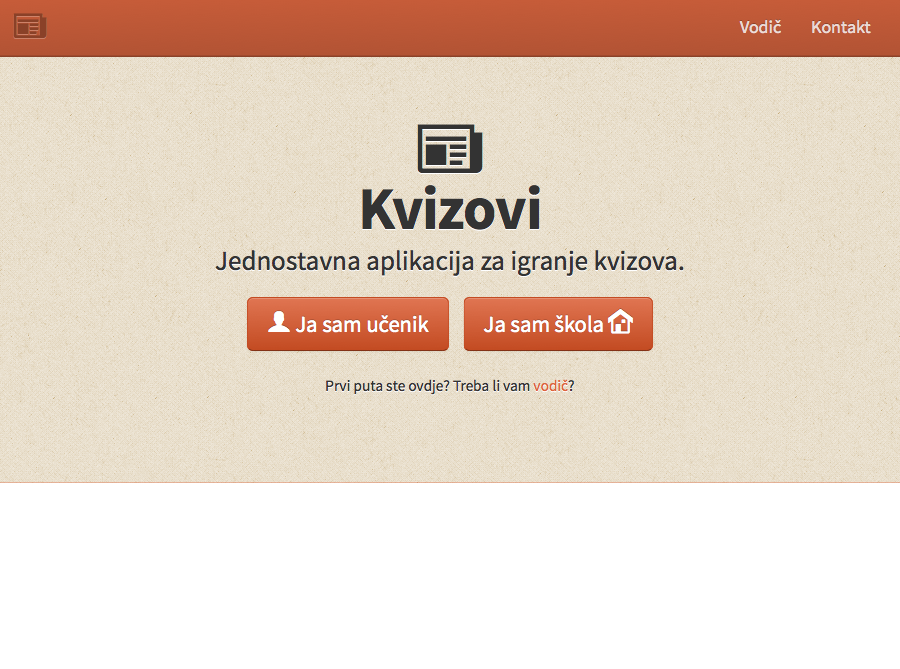
\includegraphics[width=\textwidth, clip=true, trim=0 7cm 0 0, fbox]{home}
  \caption{Početna stranica}
  \label{fig:home}
\end{figure}

\section{Korisničko sučelje}

\subsection{Škola}

\emph{Škola} je uloga koja predstavlja profesora i ona je administrator kvizova.

% S obzirom na uzrast...

Nakon odabira te uloge korisnik se može prijaviti ili registrirati ako još nema
korisnički račun. Registracija se sastoji od ispunjavanja jednostavnog formulara
pomoću kojega skupljamo informacije o korisnicima koje možemo iskoristiti kako
bismo poboljšali njihovo iskustvo i kako bismo mogli raditi istraživanja. Polje
u formularu za registraciju na koje ćemo se osvrnuti je \emph{Tajni ključ}, koji
je potreban za registraciju učenicima te škole.

Nakon prijave, nastavnicima se otvara stranica s popisom kvizova koje su
kreirali (vidi sliku \ref{fig:school/quizzes}),

\begin{figure}[H]
  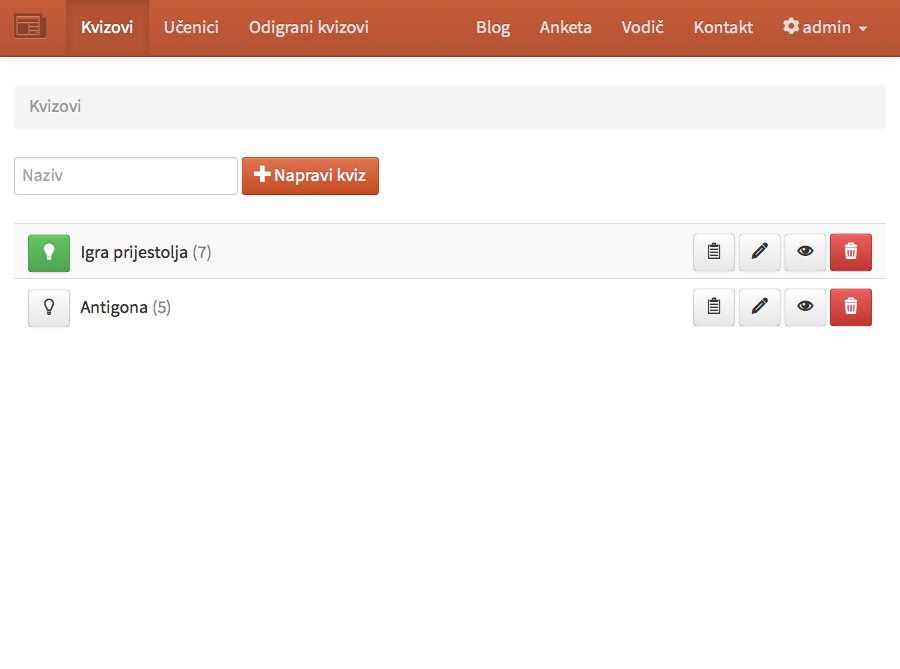
\includegraphics[width=\textwidth, clip=true, trim=0 10cm 0 0, fbox]{school/quizzes}
  \caption{Škole -- popis kvizova}
  \label{fig:school/quizzes}
\end{figure}

gdje mogu izmjenjivati postojeće kvizove i sastavljati nove. Nakon što je
profesor zadovoljan s kvizom, može ga učiniti aktivnim, odnosno vidljivim
učenicima. Izmjenjivanje kvizova podijeljeno je na izmjenu metapodataka kviza i
na izmjenu pitanja kviza. Ovdje napominjemo da ćemo, zbog zaštite privatnosti
naših korisnika, u radu prikazivati podatke kviza kojeg smo sami napravili
(Igra prijestolja), a našim imenima ćemo zamijeniti stvarna imena korisnika
koji su sudjelovali u istraživanju.

\begin{figure}[H]
  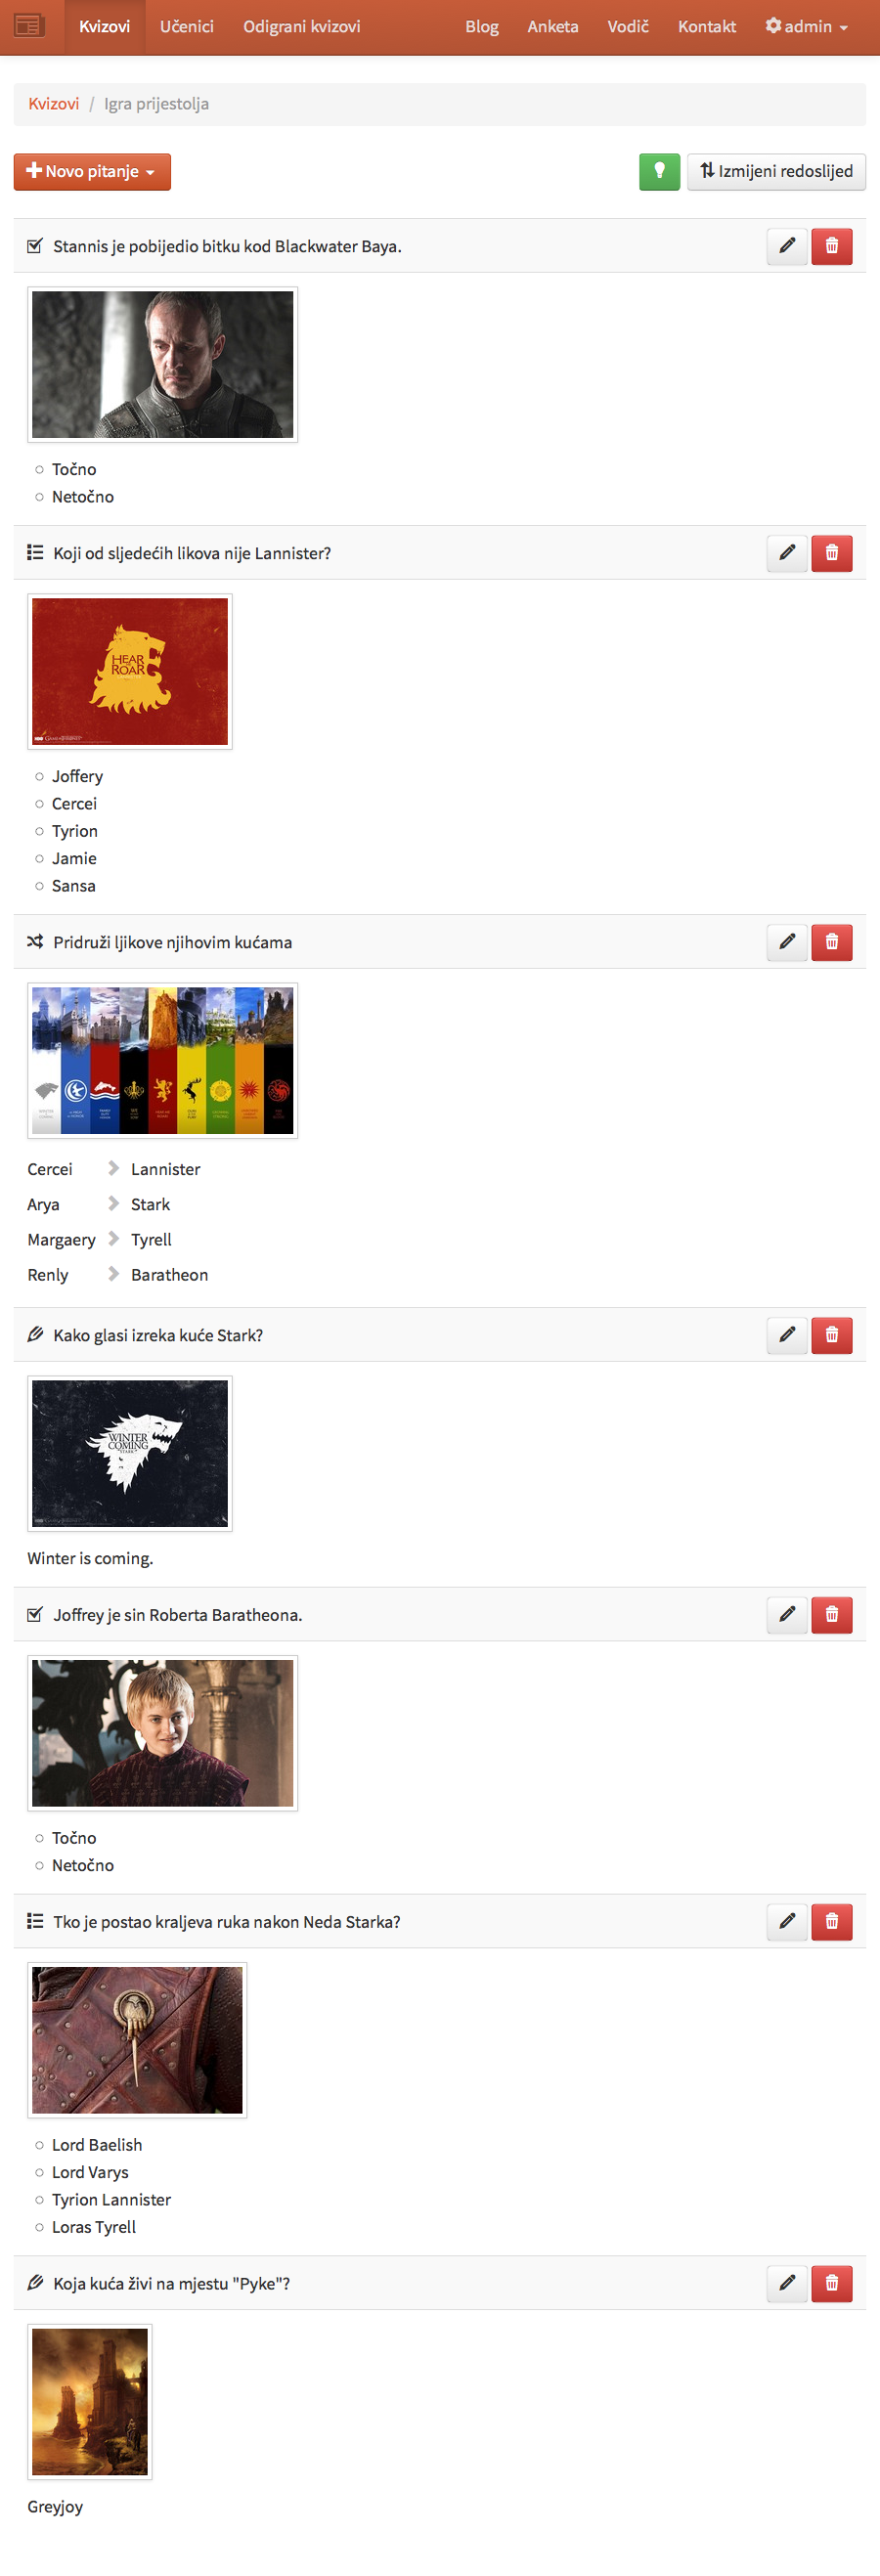
\includegraphics[width=\textwidth, clip=true, trim=0 53cm 0 0, fbox]{school/quiz}
  \caption{Škole -- popis pitanja u kvizu}
\end{figure}

Postoji 4 vrsta pitanja:

\begin{itemize}
  \item Točno/netočno
  \item Ponuđeni odgovori
  \item Asocijacija
  \item Upiši točan odgovor
\end{itemize}

Uz svako se pitanje može pridružiti pomoć (slikom ili tekstom), koja će se
prikazati učenicima dok rješavaju pitanje.

Škole mogu pregledavati informacije o odigranim kvizovima: kada su igrani, tko
ih je igrao, koji su bili rezultati itd. (vidi \ref{played_quizzes} i \ref{played_quiz}).

\begin{figure}[H]
  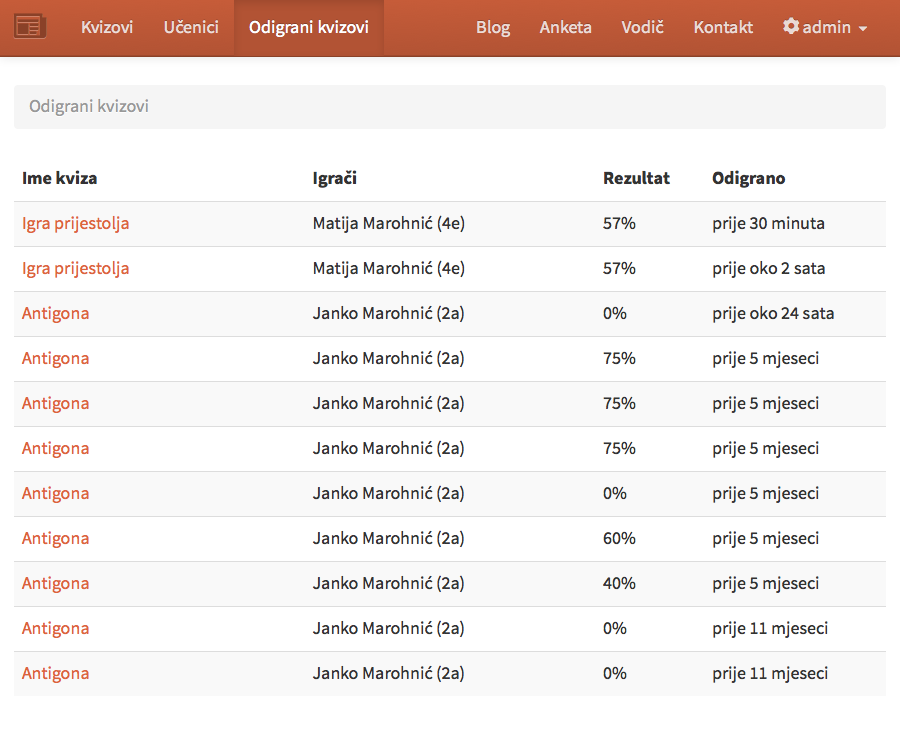
\includegraphics[width=\textwidth, clip=true, trim=0 10cm 0 0, fbox]{school/played_quizzes}
  \caption{Škole -- popis odigranih kvizova}
  \label{played_quizzes}
\end{figure}

\begin{figure}[H]
  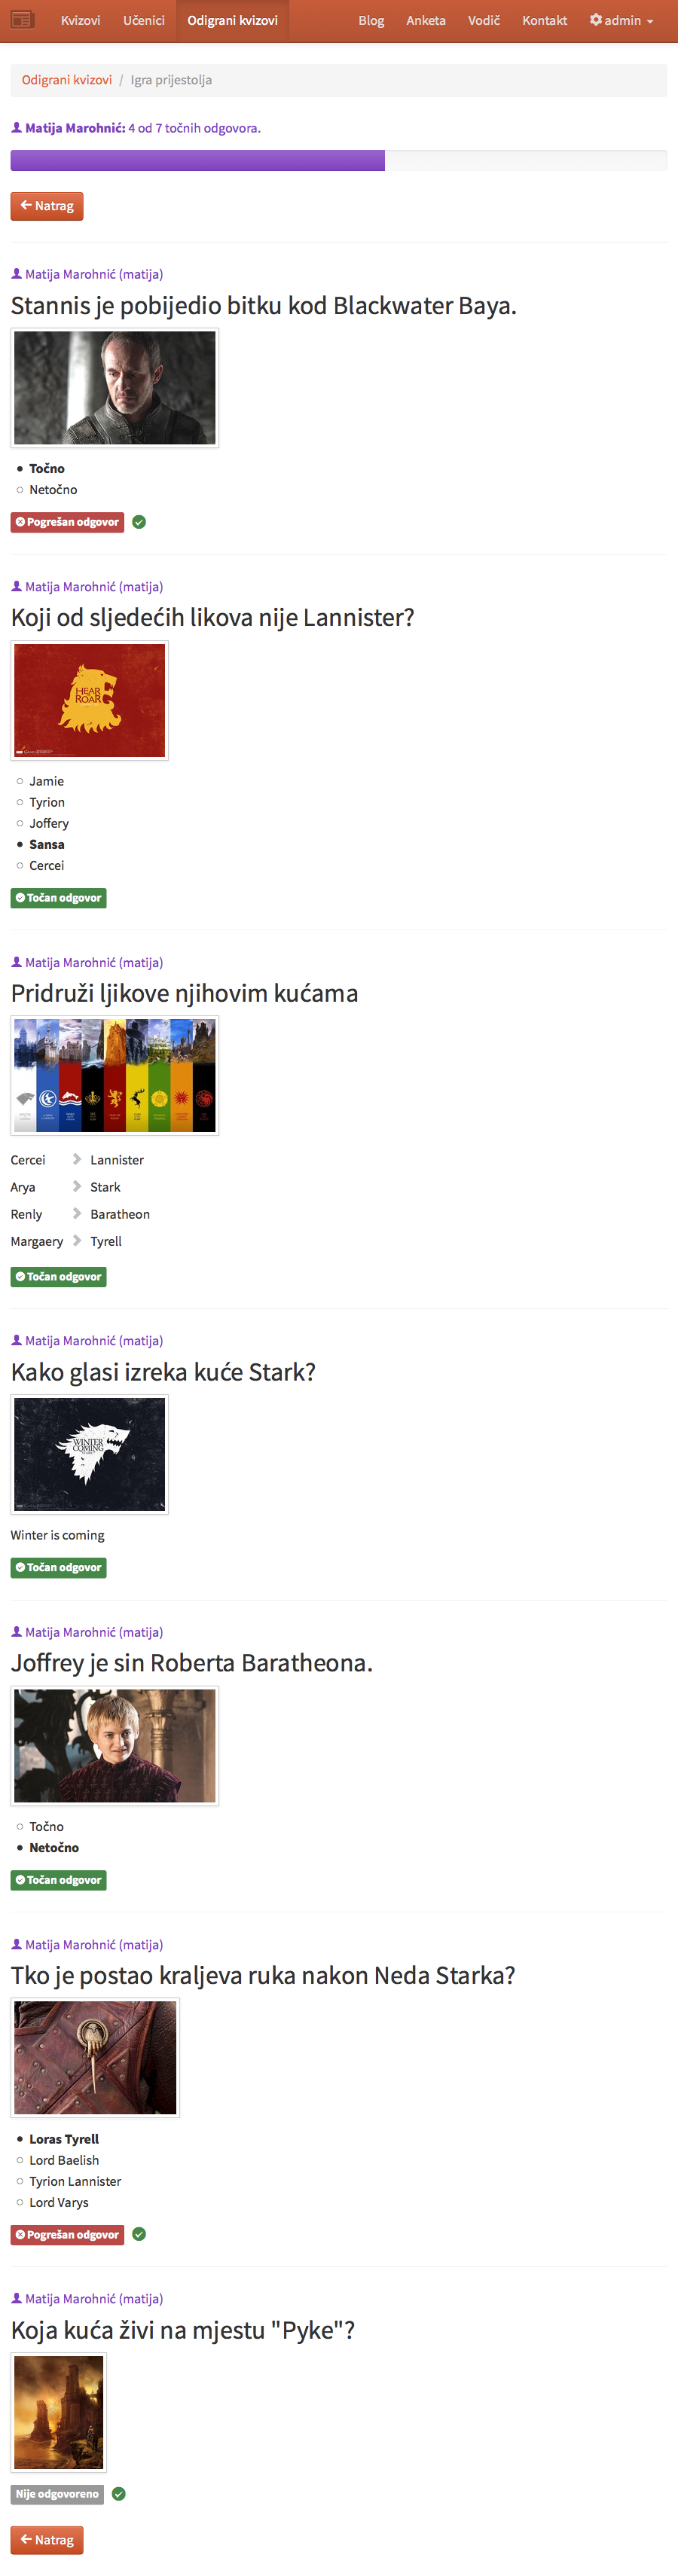
\includegraphics[width=\textwidth, clip=true, trim=0 80cm 0 0, fbox]{school/played_quiz}
  \caption{Odigrani kviz}
  \label{played_quiz}
\end{figure}

Mogu se pregledavati i učenici, koliko su kvizova odigrali, koji su to kvizovi i
sl. (vidi sliku \ref{students}).

\begin{figure}[H]
  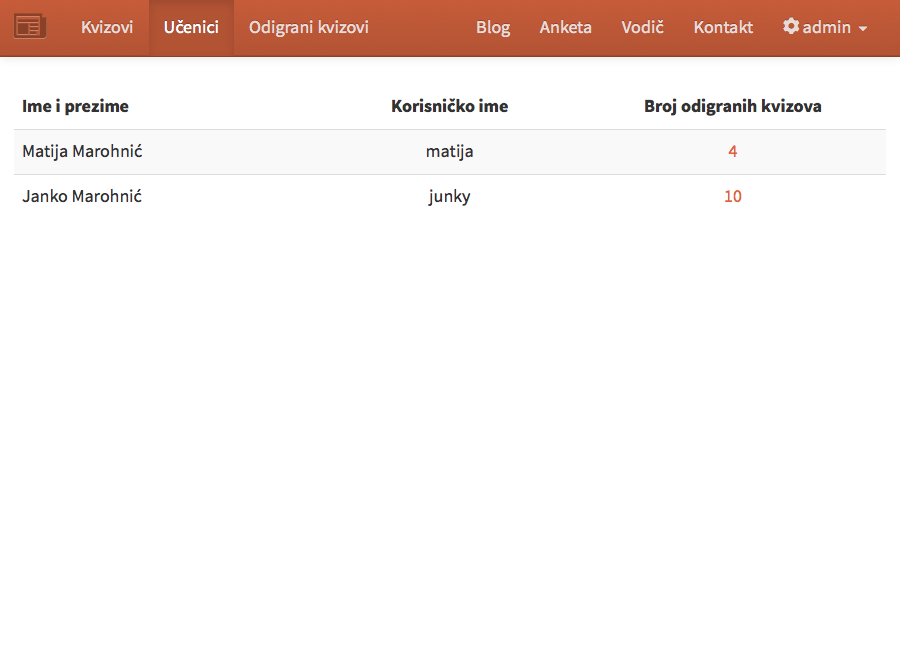
\includegraphics[width=\textwidth, clip=true, trim=0 15cm 0 0, fbox]{school/students}
  \caption{Škole -- popis učenika}
  \label{students}
\end{figure}

\subsection{Učenik}

% S obzirom na uzrast...

\emph{Učenik} je uloga koja rješava kvizove koje je napravila njihova škola.
Kao i kod škole, učenik se može prijaviti ili registrirati, ako već nema
korisnički račun. Pri registraciji učenik treba napisati tajni ključ koji mu je
njegova škola dala, u protivnom se ne može registrirati. Na taj način
sprječavamo da se bilo tko registrira kao učenik.

Nakon prijave ili registracije, korisnika dočeka lista kvizova koji su dostupni
za rješavanje. Kviz je moguće igrati samostalno ali i u paru (vidi sliku
\ref{student/quizzes}). U drugom slučaju, drugi igrač također mora biti prijavljen
u sustav.

\begin{figure}[H]
  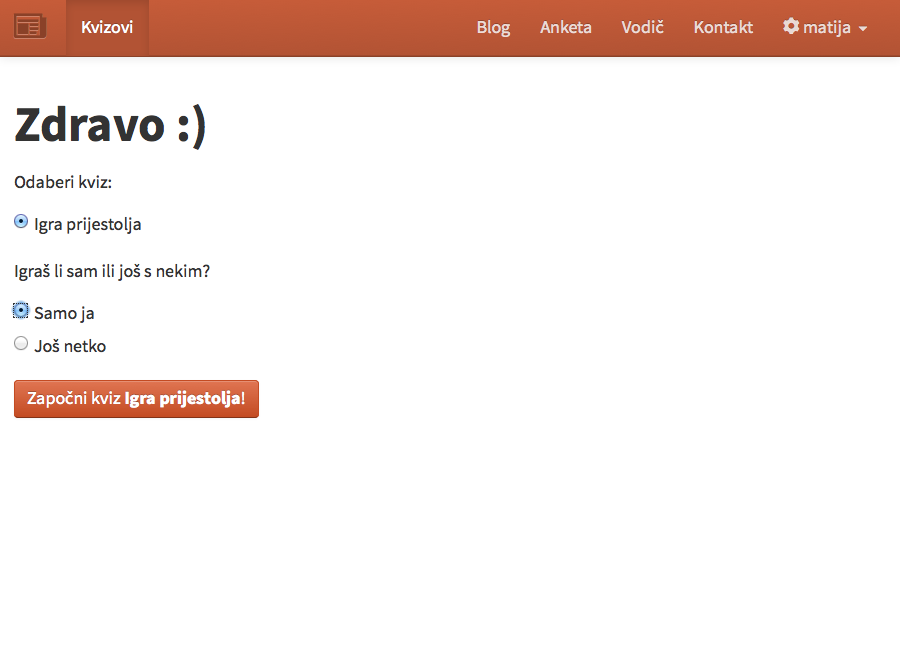
\includegraphics[width=\textwidth, clip=true, trim=0 8.5cm 0 0, fbox]{student/quizzes}
  \caption{Učenici -- popis kvizova}
  \label{student/quizzes}
\end{figure}

Nakon što učenik započne kviz, prikazuje mu se jedno po jedno pitanje na koja
treba odgovoriti. Kako bi igra bila što poštenija, pitanja su obično vremenski
ograničena, tako da se učenik ne stigne previše konzultirati s vanjskim
izvorima. Preostalo vrijeme ispisano je iznad imena korisnika (vidi sliku
\ref{question}).

\begin{figure}[H]
  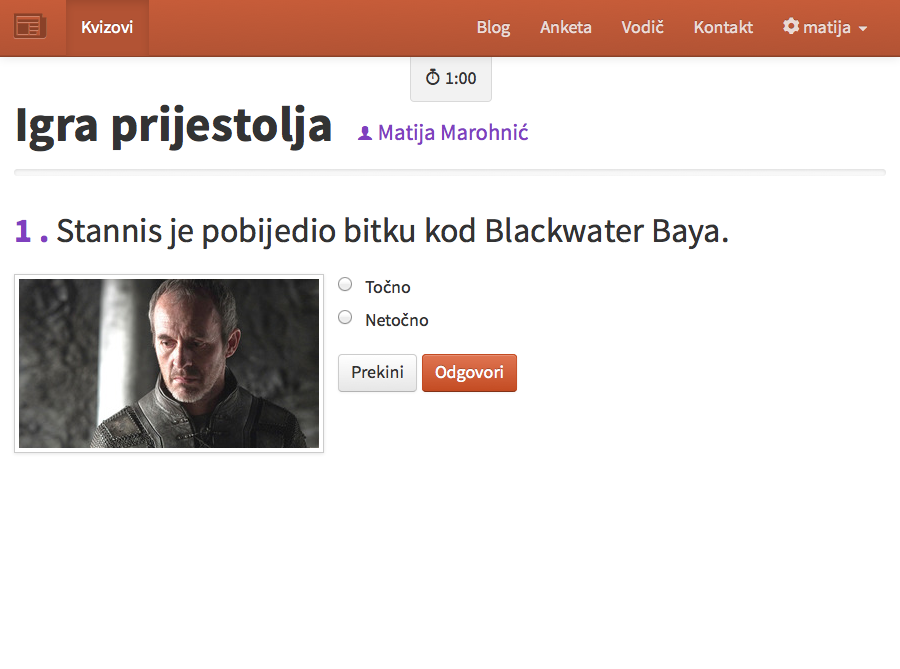
\includegraphics[width=\textwidth, clip=true, trim=0 7cm 0 0, fbox]{student/boolean_question}
  \caption{Učenici -- odgovaranje na pitanje}
  \label{question}
\end{figure}

\begin{figure}[H]
  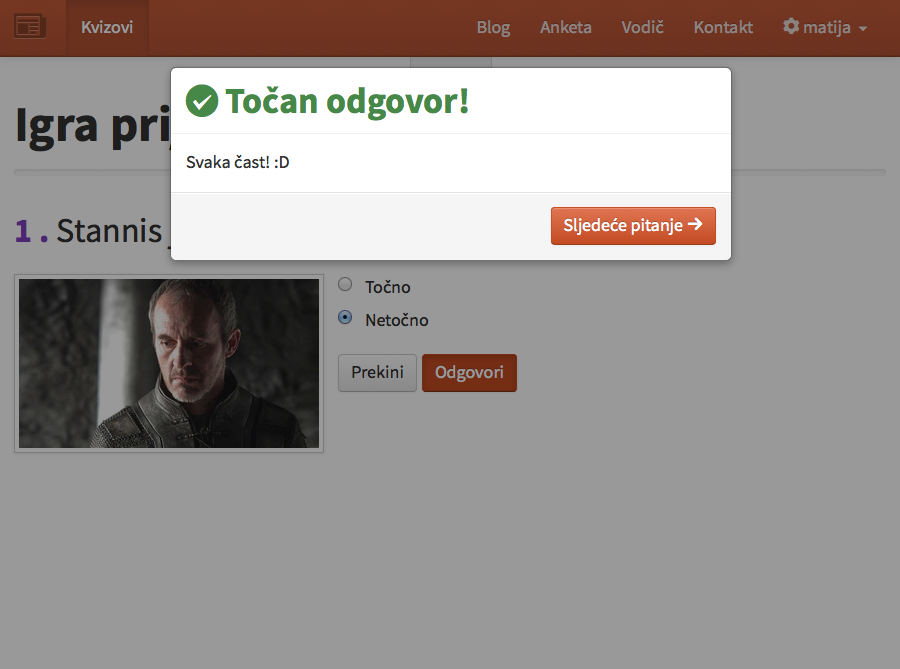
\includegraphics[width=\textwidth, clip=true, trim=0 7cm 0 0, fbox]{student/boolean_question_correct}
  \caption{Učenici -- povratna informacija nakon predanog odgovora}
\end{figure}

Nakon što učenik odgovori na sva pitanja, ispisuju se rezultati i učenik dobiva
određenu ``titulu'' s obzirom na njegov rezultat:

\begin{description}
  \item[Znalac-malac] 0\%-30\% točnih odgovora
  \item[Ekspert] 30\%-70\% točnih odgovora
  \item[Super-ekspert] 70\%-100\% točnih odgovora
\end{description}

Titule su osmišljene zato da se učenika uvijek pohvaljuje, čak i ako je imao loš
rezultat, tako da se učenik dobro osjeća i da ga se potiče da igra i dalje.

\section{Tehnologija}

Naš je cilj napraviti aplikaciju koja će raditi dobro na svim uređajima, na
mobilnim uređajima, na laptopima i na desktop računalima.\footnote{Trenutno
nemamo podršku za mobilne uređaje, pa korisničko iskustvo na njima ne bi bilo
dobro zbog nedovoljne prilagodbe dimenzija aplikacije njihovom ekranu.}
\emph{Kvizovi} su web aplikacija, dakle sa strane klijenta (web preglednika)
koristimo tehnologije kao što su HTML5, CSS3 i JavaScript. Sa strane
poslužitelja koristimo programski jezik Ruby, a kao bazu podataka relacijsku
bazu PostgreSQL.

\chapter{Rezultati}

Ovo istraživanje pokazalo je da je većina profesora primijetila napredak u
poznavanju gradiva kod svojih učenika, kao i veću zainteresiranost za gradivo.

\begin{figure}[H]
  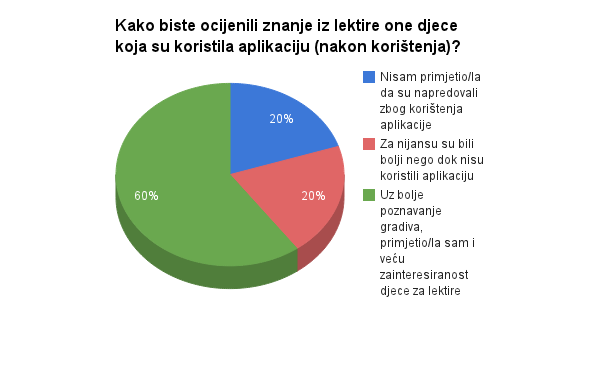
\includegraphics[width=\textwidth, clip=true, trim=0 2.5cm 0 0]{advance}
  \caption{Napredak učenika}
\end{figure}

\begin{figure}[H]
  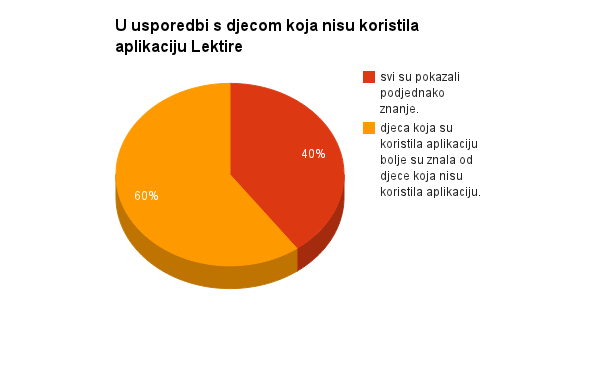
\includegraphics[width=\textwidth, clip=true, trim=0 2.5cm 0 0]{comparison}
  \caption{Usporedba učenika koji su koristili aplikaciju s onima koji nisu}
\end{figure}

\chapter{Zaključak}

Tijekom izrade ove aplikacije uočili smo mnogo načina na koje bismo mogli
poboljšati aplikaciju. Već radimo i na novim promjenama s namjerom poboljšanja
projekta, a koje su proizašle iz dobivenih rezultata rješavanja kvizova i
ispunjavanja anketa. Aplikacija \emph{Kvizovi} je inicijalno nastala kao pomoćno
sredstvo za učenje lektira, ali više ne vidimo razlog zašto se aplikacija ne bi
koristila i za ostale školske predmete kao što su zemljopis, biologija, kemija
itd.

Radimo na tome da sučelje aplikacije bude dovoljno jednostavno da vodič za
aplikaciju više neće biti potreban, već da je jasno samo po sebi kako postići
određeni cilj. Iako aplikaciju koriste stariji profesori koji nisu vješti u
korištenju aplikacije, vjerujemo da korisnici više vole učiti kako koristiti
aplikaciju iz prakse, a ne čitajući upute i da aplikaciju možemo učinit dovoljno
jednostavnom da je pristupačna za svaki uzrast i stupanj informatičke
obrazovanosti.

\chapter{Zahvale}

Htjeli bismo zahvaliti našoj mentorici, prof. dr. sc. Kristini Kocijan na ideji
aplikacije \emph{Kvizovi}, strukturiranju ovoga rada i na prikupljanju uzorka
škola koje su bile voljne koristiti našu aplikaciju i pomoći nam kod
istraživanja. Nadalje, htjeli bismo zahvaliti profesorima i učenicima iz uzorka
na sudjelovanju u ovom istraživanju i na slanju prijedloga i prijavu grešaka,
što nam je puno pomoglo u razvijanju aplikacije.

Sortirane prema broju aktivnih kvizova, škole koje su sudjelovale u istraživanju
su: I. gimnazija, Osnovna škola Bogumila Tonija, Osnovna škola Stjepana Radića,
Srednja škola Metković, Osnovna škola Poreč, Osnovna škola Stubičke Toplice,
Gimnazija Sesvete, Poljoprivredna škola, Srednja škola ``Ivan Seljanec''
Križevci, Gimnazija fra Dominika Mandica, Medicinska škola Varaždin, Srednja
škola Čakovec, Tehnička škola Šibenik, Privatna srednja ekonomska škola INOVA,
Škola za umjetnost, dizajn, grafiku i odjeću, Zabok, Gimnazija i strukovna
škola Jurja Dobrile, Nadbiskupska klasična gimnazija.

\renewcommand{\listoffigures}{\begingroup
\tocchapter
\tocfile{\listfigurename}{lof}
\endgroup}

\listoffigures

\renewcommand{\bibname}{Popis literature}

\begin{thebibliography}{9}

  \bibitem{perisic13} Perišić, Kristina. “Kako poboljšati koncentraciju djeteta?”
    Klokanica.hr, May 21, 2013.
    \url{http://www.klokanica.hr/skolarci/skola/kako-poboljsati-koncentraciju-djeteta-168}.

  \bibitem{clark11} Clark, Donald. “Visual, Auditory, and Kinesthetic Learning
    Styles (VAK).” The Performance Juxtaposition, December 7, 2011.
    \url{http://www.nwlink.com/~donclark/hrd/styles/vakt.html}.

\end{thebibliography}

\chapter{Sažetak}

\textbf{Ključne riječi}:

\chapter{Summary}

\textbf{Keywords}:

\end{document}
